% Created 2021-01-05 Tue 21:12
% Intended LaTeX compiler: pdflatex
\documentclass[11pt]{article}
\usepackage[utf8]{inputenc}
\usepackage[T1]{fontenc}
\usepackage{graphicx}
\usepackage{grffile}
\usepackage{longtable}
\usepackage{wrapfig}
\usepackage{rotating}
\usepackage[normalem]{ulem}
\usepackage{amsmath}
\usepackage{textcomp}
\usepackage{amssymb}
\usepackage{capt-of}
\usepackage{hyperref}
\usepackage{ntheorem}
\author{nicholas martin\thanks{nmartin84@gmail.com}}
\date{\today}
\title{P-Values explained by Data Scientist}
\hypersetup{
 pdfauthor={nicholas martin},
 pdftitle={P-Values explained by Data Scientist},
 pdfkeywords={},
 pdfsubject={},
 pdfcreator={Emacs 28.0.50 (Org mode 9.5)}, 
 pdflang={English}}
\begin{document}

\maketitle
\tableofcontents

source: \href{https://towardsdatascience.com/p-values-explained-by-data-scientist-f40a746cfc8}{P-values Explained By Data Scientist | by Admond Lee | Towards Data Science}

\section*{What are P-Values?}
\label{sec:org613448c}

The Wikipedia explanation for what probability values are:
\begin{quote}
In statistical hypothesis testing, the p-value or probability value is, for a
given statistical model, the probability that, when the null hypothesis is true,
the statistical summary (such as the absolute value of the sample mean
difference between two compared groups) would be greater than or equal to the
actual observed results.
— Wikipedia
\end{quote}

There are 4 break-outs to hypothesis testing which will be covered in this
document:

\subsection*{Hypothesis Testing}
\label{sec:org3f24929}
\href{../.attach/e6/622552-cc02-418e-838f-3137ba5a7798/\_20210103\_1827150*XqFCVZreewh3lATA.png}{\_20210103\_1827150*XqFCVZreewh3lATA.png}

Our ultimate goal is to determine the statistical significance of our results,
and this is where [[\href{../202101031336-hypothesis\_testing.org}{hypothesis testing}]] comes into play. Statistical
significance is built on 3 simple ideas:
\begin{enumerate}
\item Hypothesis Testing
\item Normal Distribution
\item P-Values
\end{enumerate}

When it comes to Hypothesis testing, there are a couple terms you should be
familiar with:
\begin{description}
\item[{Null Hypothesis}] This is what we are testing that is made about a population
with sample data. Generally your null hypothesis is going to align with what
we believe is already true.
\item[{Alternative Hypothesis}] Is the one you would believe if the null hypothesis
turns out to be false, or not true. This is generally what you suspect has
changed, and testing to see if this is likely or possible.
\end{description}

Basically we will make a claim (null hypothesis), and use our sample data to
test and see if it's true.

Part of this process involves calculating our confidence level, our confidence
to prove something true or not. For this we'll say for example we're looking for
a 95\% confidence level.

To know if the null hypothesis is true or not, we use the \textbf{p-value} as a weight to
see if it's statistically significant. However, if the evidence supports the
alternative hypothesis, then we'll go with that.

For an example let's say we are looking at delivery times from a pizza place
which claims they deliver in 30 minutes or under, however we think this is not
true and their delivery times are over 30 minutes.

\begin{description}
\item[{Your null hypothesis would be}] Delivery times are 30 minutes or less.
\item[{Your alternative hypothesis would be}] Delivery times are greater than 30 minutes.
\end{description}

The goal here is to determine which claim — the null or alternative — is better
supported by the evidence found from our sample data.

For this, we will use a [[\href{../202101031837-one\_tailed\_test.org}{one-tailed test}]] since we only care if the mean is
above 30 minutes. One of the common ways of testing is to use a [[\href{../202101031841-z\_test.org}{Z-Test}]], more
details on that can come later.

TODO Read the article on Z-Test and update this section, or the Z-Test article
to cover details.

\subsection*{Normal Distribution}
\label{sec:org85e31d4}
\href{../.attach/6d/949153-db6f-4802-8248-e155309e61b9/\_20210103\_1843100*\_CpITbEtFQZD45bX.png}{\_20210103\_1843100*\_CpITbEtFQZD45bX.png}

Normal distribution is a [[\href{../202101031947-probability\_density\_function.org}{probability density function}]] used to see the data
distribution.

The normal distribution has two parameters — the mean (μ) and [[\href{../202101031954-standard\_deviation.org}{standard deviation}]], also called sigma (σ).

The mean is the central tendency of the distribution. It defines the location of
the peak for normal distributions. The standard deviation is a measure of
variability. It determines how far away from the mean the values tend to fall.

The normal distribution is commonly associated with the [[\href{../202101032023-68\_95\_99\_7\_rule.org}{68-95-99.7 rule}]]
(image above).
\begin{enumerate}
\item 68\% of the data is within 1 standard deviation (σ) of the mean (μ)
\item 95\% of the data is within 2 standard deviations (σ) of the mean (μ)
\item 99.7\% of the data is within 3 standard deviations (σ) of the mean (μ)
\end{enumerate}

The [[\href{../202101032041-five\_sigma.org}{five sigma}]] threshold for discovering the \textbf{Higgs Boson} is about a
99.9999426696856\% of the data to hit before scientists confirmed the discovery
of Higgs Boson. That was the [[\href{../202101032043-stringent\_threshold.org}{stringent threshold}]] set to avoid any potential
false signals.

So next, we need to calculate Z-scores (to be used in our test-statistic) which
is the number of [[\href{../202101031954-standard\_deviation.org}{standard deviation}]] from the mean a data point is. In our case,
each data point is the pizza delivery time that we collected.

standardized the variable by subtracting the mean and dividing by its standard deviation.
\[ z
  = \frac{x-\mu}{\sigma}
\]

Looking at the standard normal distribution curve is useful because we can
compare results from a test to a “normal” population with a standardized unit in
standard deviation, especially when we have a variable that comes with different
units.

A Z-score can tell us where the overall data lies compared to the average population.

\begin{center}
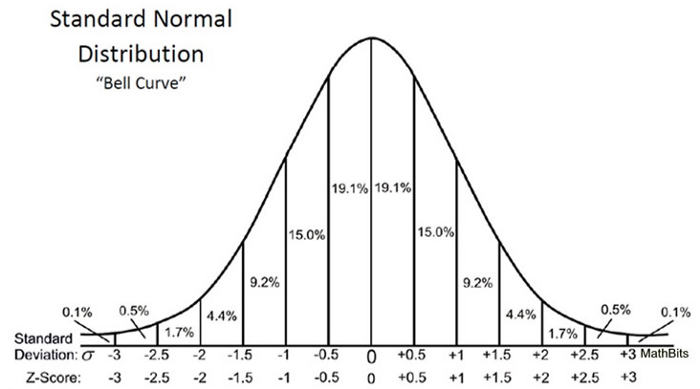
\includegraphics[width=.9\linewidth]{../.attach/6d/949153-db6f-4802-8248-e155309e61b9/_20210103_2124331*N1GR0w1rk3R0XZYrOUSwLQ.png}
\end{center}

\begin{quote}
The higher or lower the Z-score, the more unlikely the result is to happen by
chance and the more likely the result is meaningful.
\end{quote}

But that raises the question: \textbf{But how high (or low) is considered as
sufficiently convincing to quantify how meaningful our results are?}

This is where \textbf{P-Values} come into play, and check if our results are
statistically significant based on the [[\href{../202101032129-significance\_level.org}{significance level}]] (also known as alpha).

\subsection*{What is P-Value?}
\label{sec:org8f86f41}

So basically our p-value is the probability, to indicate how likely it is that
our data could be true. It's like saying, ok you're answer holds 10\%
creditability, or is 90\% crazy so we're rejecting it.

Where on the other hand, your p-value is .87 (87\%), then it holds more
significance to our null hypothesis being true.

It's important to also remember, this is not saying that the \textbf{alternative}
hypothesis is true, it's just saying that the data is showing the \textbf{null
hypothesis} is likely false but it hasn't proven it yet.

\subsection*{Level of Confidence}
\label{sec:org3417419}

This is our confidence of how much we want to believe in our hypothesis to say
it's true or valid. It's basically saying, I want my data to return with a 95\%
confidence level to prove my alternative hypothesis. \[ confidence=95\% \]

\subsection*{Level of Significance}
\label{sec:org29abd62}

This is where we basically draw the line in our data to help us make a decision.

Our level of significance is basically: \[ \alpha=1-confidence \] If \(LOC=95%\)
and \(Confidence=0.95\) then our equation to find our level of significance would
be \[ \alpha=1-0.95 \] so our results would be \[ \alpha=0.05 \]

\subsection*{Conclusion of p-values}
\label{sec:orgbabb520}

So ultimately, p-value is what's being used to determine if our hypothesis holds
weight. So it comes down to the basics of:

\[ p \leq \alpha = Reject Ho \]

Otherwise:

\[ p > \alpha = Fail to Reject Ho \]
\end{document}
